\documentclass[11pt, a4paper]{article}
\usepackage[utf8]{inputenc}
\usepackage[T1]{fontenc}
\usepackage{amsmath, amssymb, amsthm}
\usepackage{algorithm}
\usepackage{algpseudocode}
\usepackage{algorithmicx}
\usepackage{tikz}
\usetikzlibrary{positioning,arrows.meta}
\usepackage{geometry}
\usepackage{hyperref}
\usepackage{minted}
\setminted{style=friendly, fontsize=\small, breaklines=true, linenos=true, bgcolor=gray!6, numbersep=8pt}
\usepackage{float}
\usepackage{xcolor}
\usepackage{booktabs}
\usepackage{parskip}
\usepackage{mathtools}

\geometry{margin=2.5cm}


\title{\textbf{Gradient Boosting from Scratch} \\[6pt]
       }
\author{Jason Jang}
\date{}

\begin{document}
\maketitle

\begin{abstract}
This document builds modern gradient boosting from the ground up, assuming only
undergraduate calculus (derivatives, chain rule, Taylor expansion).
We derive every equation step by step, implement each component in
pure NumPy, and map every line of code back to its mathematical origin.
Starting from Vanilla GBM, we introduce five innovations in sequence ---
Newton Step, Oblivious Trees, Ordered Target Statistics, Ordered Boosting,
and Posterior Sampling (SGLB) --- each motivated by a concrete limitation
of the previous approach.
Source code: \texttt{github.com/jasonjang1224/Gradient-Boosting-from-Scratch}.
\end{abstract}

\subsection*{Notation}

\begin{center}
\begin{tabular}{ll}
\toprule
\textbf{Symbol} & \textbf{Meaning} \\
\midrule
$i$ & sample index ($i = 1,\ldots,N$) \\
$f$ & feature index ($f = 1,\ldots,F$) \\
$t$ & boosting iteration index ($t = 1,\ldots,T$) \\
$d$ & tree depth level ($d = 0,\ldots,D-1$) \\
$x_i \in \mathbb{R}^F$ & feature vector of sample $i$ \\
$x_{i,f}$ & value of feature $f$ for sample $i$ \\
$y_i$ & target value of sample $i$ \\
$F_t$ & ensemble model after $t$ iterations \\
$h_t$ & single tree fitted at iteration $t$ \\
$g_i^t$ & positive gradient $\partial L(y_i,F_i)/\partial F_i$ of sample $i$ at iteration $t$ \\
$r_i^t$ & pseudo-residual $r_i = -g_i$ (negative gradient) of sample $i$ at iteration $t$ \\
$h_i^t$ & Hessian of sample $i$ at iteration $t$ \\
$\tau$ & split threshold (a real-valued scalar) \\
$(f^*, \tau^*)$ & optimal feature and threshold found by split search \\
$(f_d, \tau_d)$ & shared split at depth $d$ of an Oblivious Tree \\
$R_j$ & leaf region $j$ \\
$\gamma_j$ & leaf value in region $R_j$ \\
$\sigma$ & random permutation of $\{1,\ldots,N\}$ \\
$\hat{x}_{i,f}$ & Ordered TS encoding of feature $f$ for sample $i$ \\
\bottomrule
\end{tabular}
\end{center}


% ═══════════════════════════════════════════════
\section{Background: What Problem Are We Solving?}
% ═══════════════════════════════════════════════

We have a dataset $\{(x_i, y_i)\}_{i=1}^N$ where $x_i \in \mathbb{R}^F$
are features and $y_i \in \mathbb{R}$ are targets.
We want to find a function $F: \mathbb{R}^F \to \mathbb{R}$ that
minimizes the average loss:

\[
\mathcal{L}(F) = \sum_{i=1}^N L\!\left(y_i,\, F(x_i)\right)
\]

For regression we use \textbf{Mean Squared Error}:
$L(y, \hat{y}) = \tfrac{1}{2}(y - \hat{y})^2$.

The factor $\tfrac{1}{2}$ is a convenience that cancels the $2$ from
differentiation, but does not affect the minimizer.

We are not looking for a single parametric function (like a linear model).
Instead, we will build $F$ as a \emph{sum of many small decision trees},
each correcting the mistakes of the previous ones.
This is the core idea of \textbf{boosting}.

% ═══════════════════════════════════════════════
\section{Vanilla Gradient Boosting Machine}
% ═══════════════════════════════════════════════

\subsection{Gradient Descent in Function Space}

You may be familiar with gradient descent for a parameter vector $\theta$:

\[
\theta \leftarrow \theta - \alpha \cdot \nabla_\theta \mathcal{L}
\]

GBM does the same thing, but the ``parameter'' being updated is the
\emph{function} $F$ itself. We treat $F(x_i)$, the prediction at each
training point, as a variable we want to optimize.

The gradient of $\mathcal{L}$ with respect to $F(x_i)$ is simply
the partial derivative treating $F(x_i)$ as a scalar:

\[
\frac{\partial \mathcal{L}}{\partial F(x_i)}
= \frac{\partial}{\partial F(x_i)} \sum_j L(y_j, F(x_j))
= \frac{\partial L(y_i, F(x_i))}{\partial F(x_i)}
\]

(All other terms vanish because they do not depend on $F(x_i)$.)

Let $g_i^t = \partial L(y_i, F_{t-1}(x_i))/\partial F_{t-1}(x_i)$ be the
\textbf{positive gradient} (first derivative of loss with respect to the prediction).
The \textbf{pseudo-residual} is the negative gradient:
\[
r_i^t = -g_i^t = -\frac{\partial L(y_i, F(x_i))}{\partial F(x_i)}\bigg|_{F = F_{t-1}}
\]

\textbf{MSE case.}
$L(y_i, F_i) = \tfrac{1}{2}(y_i - F_i)^2$, so:
\[
g_i^t = \frac{\partial L}{\partial F_i} = F_i - y_i
\quad\Rightarrow\quad
r_i^t = -g_i^t = y_i - F_{t-1}(x_i)
\]

The pseudo-residual $r_i^t = y_i - F_{t-1}(x_i)$ is the residual (prediction error).
Fitting trees to pseudo-residuals $r_i^t$ is equivalent to taking a step in the
negative gradient direction in function space.

\begin{listing}[H]
\caption{Pseudo-residual computation (\texttt{vanilla\_gbm.py})}
\begin{minted}[linenos, bgcolor=gray!6, fontsize=\small, breaklines]{python}
def _get_gradients(self, y, F_pred):
    # r_i = y_i - F_{t-1}(x_i)  (pseudo-residual = negative gradient)
    # For MSE: g_i = F_i - y_i, so r_i = -g_i = y_i - F_i
    return y - F_pred        # shape (N,)
\end{minted}
\end{listing}

\subsection{Initialization}

Before the first tree, we predict a constant $F_0$ for all samples.
The optimal constant minimizes the total loss:

\[
F_0 = \operatorname{arg\,min}_\gamma \sum_{i=1}^N L(y_i, \gamma)
\]

For MSE, take the derivative with respect to $\gamma$ and set it to zero:

\[
\frac{d}{d\gamma} \sum_{i=1}^N \tfrac{1}{2}(y_i - \gamma)^2
= -\sum_{i=1}^N (y_i - \gamma) = 0
\quad\Rightarrow\quad
\boxed{F_0 = \bar{y} = \frac{1}{N}\sum_{i=1}^N y_i}
\]

\begin{listing}[H]
\caption{Initialization (\texttt{vanilla\_gbm.py})}
\begin{minted}[linenos, bgcolor=gray!6, fontsize=\small, breaklines]{python}
def _initialize(self, y):
    # F_0 = mean(y): the optimal constant prediction under MSE.
    # Derivation: argmin_gamma sum (y_i - gamma)^2
    #             d/d(gamma) = -2 * sum(y_i - gamma) = 0
    #             => gamma* = mean(y)
    return np.mean(y)
\end{minted}
\end{listing}

\subsection{Fitting a Tree to Pseudo-residuals}

Recall what we are trying to do: take one step of gradient descent in function space.
The ideal update would be to add the pseudo-residual $r_i^t = -g_i^t$ to the prediction
at every training point $x_i$, moving each prediction in the direction that reduces loss.
The problem is that this update is defined only at the $N$ training points --- it
tells us nothing about how to predict at a new, unseen $x$.

This is why we fit a \textbf{decision tree} $h_t$ to the pseudo-residuals $r_i^t$.
The tree generalises the gradient step to the entire input space: instead of
memorising $r_i^t$ at each point, it finds regions of feature space where
the pseudo-residuals are similar, and assigns a single constant to each region.
Predicting with $h_t$ at a new point $x$ is equivalent to asking
``which region does $x$ fall into, and what was the average correction
needed there during training?''

Formally, $h_t$ partitions the feature space into $J$ disjoint
leaf regions $\{R_j\}_{j=1}^J$ and outputs a constant $\gamma_j$
in each region:

\[
h_t(x) = \sum_{j=1}^J \gamma_j \cdot \mathbf{1}[x \in R_j]
\]

\subsubsection{Optimal Leaf Value}

Within leaf $R_j$, the optimal constant $\gamma_j$ minimizes the MSE
over the pseudo-residuals assigned to that leaf:

\[
\gamma_j
= \operatorname{arg\,min}_\gamma \sum_{i \in R_j} (r_i - \gamma)^2
\]

Differentiating and setting to zero (same as the $F_0$ derivation):

\[
\boxed{\gamma_j = \frac{1}{|R_j|} \sum_{i \in R_j} r_i = \bar{r}_{R_j}}
\]

The optimal leaf value is the \emph{mean pseudo-residual} in that leaf.

\begin{listing}[H]
\caption{Leaf value computation (\texttt{vanilla\_gbm.py})}
\begin{minted}[linenos, bgcolor=gray!6, fontsize=\small, breaklines]{python}
def _make_leaf(self, r):
    # gamma_j = mean(r) over leaf region R_j
    # r_i = y_i - F_i  (pseudo-residual); argmin_gamma sum(r_i - gamma)^2
    node = Node()
    node.value = np.mean(r)    # gamma_j = r-bar_{R_j}
    return node
\end{minted}
\end{listing}

\subsubsection{Split Gain Derivation}

How do we choose \emph{which} feature and threshold to split on?
We want the split that most reduces the total MSE over pseudo-residuals.

A split on feature $f$ at threshold $\tau$ creates:
\[
R_1 = \{i : x_{i,f} \leq \tau\},\quad R_2 = \{i : x_{i,f} > \tau\}
\]

The MSE in a region $R$ with optimal leaf value $\bar{r}_R$ is:
\[
\mathrm{MSE}(R) = \sum_{i \in R} (r_i - \bar{r}_R)^2
\]

Expanding the square:
\[
\mathrm{MSE}(R)
= \sum_{i \in R} r_i^2 - 2\bar{r}_R \sum_{i \in R} r_i + |R|\bar{r}_R^2
= \sum_{i \in R} r_i^2 - |R|\bar{r}_R^2
\]

where we used $\bar{r}_R = \frac{1}{|R|}\sum_{i\in R}r_i$, so
$|R|\bar{r}_R^2 = \frac{(\sum_{i\in R}r_i)^2}{|R|}$.

We define the \textbf{split gain} as the reduction in total MSE achieved
by the split:
\[
\mathrm{Gain}(f,\tau)
= \mathrm{MSE}(\text{parent}) - \bigl[\mathrm{MSE}(R_1) + \mathrm{MSE}(R_2)\bigr]
\]

We want to choose the split that \emph{maximizes} this reduction.
Substituting the expanded form of $\mathrm{MSE}(R)$:
\begin{align*}
\mathrm{Gain}(f,\tau)
&= \Bigl[\textstyle\sum_i r_i^2 - \tfrac{(\sum_i r_i)^2}{N}\Bigr]
 - \Bigl[\textstyle\sum_{i\in R_1} r_i^2 - \tfrac{(\sum_{i\in R_1}r_i)^2}{|R_1|}\Bigr]
 - \Bigl[\textstyle\sum_{i\in R_2} r_i^2 - \tfrac{(\sum_{i\in R_2}r_i)^2}{|R_2|}\Bigr]
\end{align*}

The $\sum r_i^2$ terms cancel (parent = $R_1 \cup R_2$, disjoint), leaving:

\[
\mathrm{Gain}(f,\tau) =
\frac{\Bigl(\displaystyle\sum_{i \in R_1} r_i\Bigr)^2}{|R_1|}
+\frac{\Bigl(\displaystyle\sum_{i \in R_2} r_i\Bigr)^2}{|R_2|}
-\frac{\Bigl(\displaystyle\sum_{i} r_i\Bigr)^2}{N}
\]

The third term is the \textbf{baseline score} (parent MSE contribution).
It is subtracted so that $\mathrm{Gain} > 0$ only when splitting actually helps.

Why subtract the baseline? Without it, any split would always look beneficial,
because $\frac{A^2}{n_1} + \frac{B^2}{n_2} \geq \frac{(A+B)^2}{n_1+n_2}$
by the Cauchy--Schwarz inequality (equality holds only when $A/n_1 = B/n_2$,
i.e.\ the split produces two perfectly balanced groups with identical means ---
which means the split does nothing useful).
Subtracting the baseline makes $\mathrm{Gain} = 0$ in that degenerate case,
and $\mathrm{Gain} > 0$ only when the split genuinely separates the
pseudo-residuals. In code, \texttt{score\_no\_split = sum\_t**2 / N}
is this baseline, computed once and reused across all candidate splits.

\begin{listing}[H]
\caption{Split search (\texttt{vanilla\_gbm.py})}
\begin{minted}[linenos, bgcolor=gray!6, fontsize=\small, breaklines]{python}
def _find_split(self, X, g):
    N, F = X.shape
    sum_t = g.sum()
    # Baseline: score if we do NOT split (one leaf for all)
    # = (sum g)^2 / N
    score_no_split = sum_t ** 2 / N

    best_gain, best_feature, best_threshold = 0.0, None, None

    for j in range(F):                      # try every feature
        order    = np.argsort(X[:, j])      # sort by feature value
        g_sorted = g[order]
        x_sorted = X[order, j]
        sum_L    = 0.0

        for i in range(1, N):               # try every threshold
            sum_L += g_sorted[i - 1]        # cumulative sum for left
            sum_R  = sum_t - sum_L          # right = total - left
            n_L, n_R = i, N - i

            # skip if x values are equal (no real threshold here)
            if x_sorted[i] == x_sorted[i - 1]:
                continue

            # Gain = (sum_L)^2/n_L + (sum_R)^2/n_R - baseline
            gain = sum_L**2 / n_L + sum_R**2 / n_R - score_no_split

            if gain > best_gain:
                best_gain      = gain
                best_feature   = j
                # threshold = midpoint between adjacent values
                best_threshold = (x_sorted[i - 1] + x_sorted[i]) / 2.0

    return best_feature, best_threshold, best_gain
\end{minted}
\end{listing}

\subsubsection{What is $h_t$ exactly?}

After the split search finds the best $(f^*, \tau^*)$ at each node,
the tree $h_t$ is fully defined by two things:

\begin{enumerate}
  \item \textbf{The partition.}
    The recursive splits divide the feature space into $J$ disjoint leaf
    regions $R_1, \ldots, R_J$.
    Every training sample $x_i$ falls into exactly one leaf.

  \item \textbf{The leaf values $\gamma_j$.}
    Within each leaf, the tree outputs a single constant --- the mean
    pseudo-residual $\bar{g}_{R_j}$ derived above.
\end{enumerate}

Putting these together:
\[
h_t(x) = \sum_{j=1}^J \bar{r}_{R_j} \cdot \mathbf{1}[x \in R_j]
\]

$h_t$ is \emph{not} trying to predict $y$ directly.
It is predicting the \textbf{current pseudo-residual} --- how much the existing
model $F_{t-1}$ is wrong by, in each region of feature space.
Adding $\eta \cdot h_t$ to $F_{t-1}$ nudges the predictions toward $y$,
one small step at a time.

\subsection{Model Update}

After fitting tree $h_t$, we update the model:

\[
F_t(x) = F_{t-1}(x) + \eta \cdot h_t(x)
\]

where $\eta \in (0, 1]$ is the \textbf{learning rate} (step size).
The final prediction after $T$ iterations is:

\[
F_T(x) = \underbrace{\bar{y}}_{F_0} + \eta \sum_{t=1}^T h_t(x)
\]

\begin{listing}[H]
\caption{Training loop (\texttt{vanilla\_gbm.py})}
\begin{minted}[linenos, bgcolor=gray!6, fontsize=\small, breaklines]{python}
def fit(self, X, y):
    self.F0 = self._initialize(y)               # F_0 = mean(y)
    F_pred  = np.full(len(y), self.F0)          # F_0(x_i) for all i

    for _ in range(self.n_estimators):
        r = self._get_gradients(y, F_pred)       # r_i = y_i - F_{t-1}(x_i) (pseudo-residual)

        tree = DecisionTree(max_depth=self.max_depth)
        tree.fit(X, r)                           # find t*, compute gamma_j = r-bar

        update  = tree.predict(X)               # h_t(x_i) for all i
        F_pred += self.learning_rate * update   # F_t = F_{t-1} + eta * h_t
        self.trees.append(tree)
\end{minted}
\end{listing}

\textbf{Notation clarification: $h_t$ versus $F_t$.}
These two symbols are easy to confuse because they both represent
``the model at step $t$'', but they refer to very different things:

\begin{center}
\begin{tabular}{lll}
\toprule
\textbf{Symbol} & \textbf{What it is} & \textbf{Used for} \\
\midrule
$h_t$ & The single tree trained at iteration $t$ & Correcting the current residual \\
$F_t$ & The cumulative ensemble up to iteration $t$ & Making the final prediction \\
\bottomrule
\end{tabular}
\end{center}

The relationship is $F_t = F_{t-1} + \eta \cdot h_t$, or equivalently:
\[
F_T(x) = \underbrace{\bar{y}}_{h_0 \text{ (constant)}} + \eta\,h_1(x) + \eta\,h_2(x) + \cdots + \eta\,h_T(x)
\]
Each $h_t$ is a weak learner (shallow tree fitting current residuals).
$F_T$ is the strong learner built by summing them all.
In code, \texttt{F\_pred} tracks $F_t$ and grows with each iteration,
while \texttt{tree} (i.e.\ $h_t$) is freshly created each time.

\begin{algorithm}[H]
\caption{Vanilla GBM (MSE)}
\begin{algorithmic}[1]
\Require $\{(x_i,y_i)\}_{i=1}^N$, learning rate $\eta$, number of trees $T$
\State $F_0 \leftarrow \bar{y}$ \hfill\Comment{optimal constant: \texttt{\_initialize()}}
\For{$t = 1, 2, \ldots, T$}
  \State $r_i^t \leftarrow y_i - F_{t-1}(x_i)$ for all $i$
    \hfill\Comment{pseudo-residuals ($= -g_i^t$): \texttt{\_get\_gradients()}}
  \State $(f^*, \tau^*) \leftarrow \operatorname{arg\,max}_{f,\,\tau}\,\mathrm{Gain}(f, \tau)$
    \hfill\Comment{best split: \texttt{\_find\_split()}}
  \State $\gamma_j \leftarrow \bar{r}_{R_j}$ for each leaf $j$
    \hfill\Comment{leaf values: \texttt{\_make\_leaf()}}
  \State $h_t(x) \leftarrow \sum_j \gamma_j\,\mathbf{1}[x\in R_j]$
  \State $F_t(x) \leftarrow F_{t-1}(x) + \eta\cdot h_t(x)$
    \hfill\Comment{update: \texttt{fit()} loop}
\EndFor
\State \Return $F_T$
\end{algorithmic}
\end{algorithm}

\begin{center}
\begin{tabular}{lll}
\toprule
\textbf{Step} & \textbf{Equation} & \textbf{Function} \\
\midrule
Initialization   & $F_0 = \bar{y}$ & \texttt{\_initialize()} \\
Pseudo-residuals & $r_i^t = y_i - F_{t-1}(x_i) = -g_i^t$ & \texttt{\_get\_gradients()} \\
Split search     & $(f^*,\tau^*) = \operatorname{arg\,max}_{f,\tau}\,\mathrm{Gain}(f,\tau)$ & \texttt{\_find\_split()} \\
Leaf values      & $\gamma_j = \bar{r}_{R_j}$ & \texttt{\_make\_leaf()} \\
Update           & $F_t = F_{t-1} + \eta\cdot h_t$ & \texttt{fit()} loop \\
\bottomrule
\end{tabular}
\end{center}

% ═══════════════════════════════════════════════
\section{Newton Step and General Loss}
\label{sec:newton}
% ═══════════════════════════════════════════════

\subsection{Second-Order Taylor Approximation}

When computing the optimal leaf value $\gamma_j$, instead of minimising
the exact loss, we use a \textbf{second-order Taylor approximation} around
the current prediction $F_{t-1}(x_i)$:

\[
L\!\left(y_i,\; F_{t-1}(x_i) + \gamma\right)
\approx L_i \;+\; g_i\,\gamma \;+\; \tfrac{1}{2}\,h_i\,\gamma^2
\]

where:
\begin{align*}
g_i &= \frac{\partial L(y_i, F(x_i))}{\partial F(x_i)}\bigg|_{F_{t-1}}
       \quad\text{(first derivative, gradient)} \\
h_i &= \frac{\partial^2 L(y_i, F(x_i))}{\partial F(x_i)^2}\bigg|_{F_{t-1}}
       \quad\text{(second derivative, Hessian)}
\end{align*}

Minimising the approximation over $\gamma$:
\[
\frac{d}{d\gamma}\left(L_i + g_i\gamma + \tfrac{1}{2}h_i\gamma^2\right)
= g_i + h_i\gamma = 0
\quad\Rightarrow\quad \gamma = -\frac{g_i}{h_i}
\]

Summing over all samples in leaf $R_j$:

\[
\gamma_j = -\frac{\sum_{i \in R_j} g_i}{\sum_{i \in R_j} h_i}
\]

\textbf{MSE verification.}
$g_i = F_i - y_i$, $h_i = 1$.
$\gamma_j = -\frac{\sum g_i}{|R_j|} = \frac{\sum(y_i - F_i)}{|R_j|} = \bar{r}_{R_j}$ (mean pseudo-residual).
Consistent with Vanilla GBM.

\subsection{Loss Interface}

We implement a unified interface so any loss function can be plugged in:

\begin{center}
\begin{tabular}{lcccc}
\toprule
\textbf{Loss} & $g_i$ & $h_i$ & $F_0$ & Notes \\
\midrule
MSE ($\tfrac{1}{2}(y-F)^2$) & $F_i - y_i$ & $1$ & $\bar{y}$ & regression \\
LogLoss ($-y\log p-(1-y)\log(1-p)$) & $p_i - y_i$ & $p_i(1-p_i)$ & $\log\!\frac{\bar{y}}{1-\bar{y}}$ & binary classification \\
\bottomrule
\end{tabular}
\end{center}

where $p_i = (1 + e^{-F_i})^{-1}$ is the sigmoid function.

\begin{listing}[H]
\caption{Loss functions (\texttt{loss.py})}
\begin{minted}[linenos, bgcolor=gray!6, fontsize=\small, breaklines]{python}
class MSE:
    def gradient(self, y, F):
        return F - y                      # g_i = F_i - y_i = dL/dF

    def hessian(self, y, F):
        return np.ones_like(y)            # h_i = d^2L/dF^2 = 1

    def leaf_value(self, g, h):
        return -g.sum() / h.sum()         # gamma_j = -sum(g)/sum(h)

    def init_prediction(self, y):
        return np.mean(y)                 # F_0 = mean(y)

class LogLoss:
    def gradient(self, y, F):
        p = 1.0 / (1.0 + np.exp(-F))
        return p - y                      # g_i = p_i - y_i

    def hessian(self, y, F):
        p = 1.0 / (1.0 + np.exp(-F))
        return p * (1.0 - p)             # h_i = p_i(1 - p_i)

    def leaf_value(self, g, h):
        return -g.sum() / (h.sum() + 1e-9)

    def init_prediction(self, y):
        p = np.clip(np.mean(y), 1e-7, 1 - 1e-7)
        return np.log(p / (1.0 - p))     # F_0 = log-odds
\end{minted}
\end{listing}

% ═══════════════════════════════════════════════
\section{Oblivious Trees}
% ═══════════════════════════════════════════════

\subsection{Motivation: Why Change the Tree Structure?}

A standard decision tree chooses a \emph{different} feature and threshold
at each node. This gives high flexibility but also high variance ---
the tree can overfit by memorising specific regions of the training data.

CatBoost replaces standard trees with \textbf{Oblivious Trees}:
trees in which every node at the same depth uses the \emph{same}
feature and threshold.

Think of an Oblivious Tree as a sequence of $D$ yes/no questions
applied to every sample:
\begin{enumerate}
  \item Is \texttt{age} $> 35$?
  \item Is \texttt{income} $> 50000$?
  \item Is \texttt{credit\_score} $> 700$?
\end{enumerate}
The answers (0 or 1) for each sample form a $D$-bit binary number
that directly identifies a leaf --- no traversal needed.

Figure~\ref{fig:trees} compares the two structures at depth 3.

\begin{figure}[h]
\centering
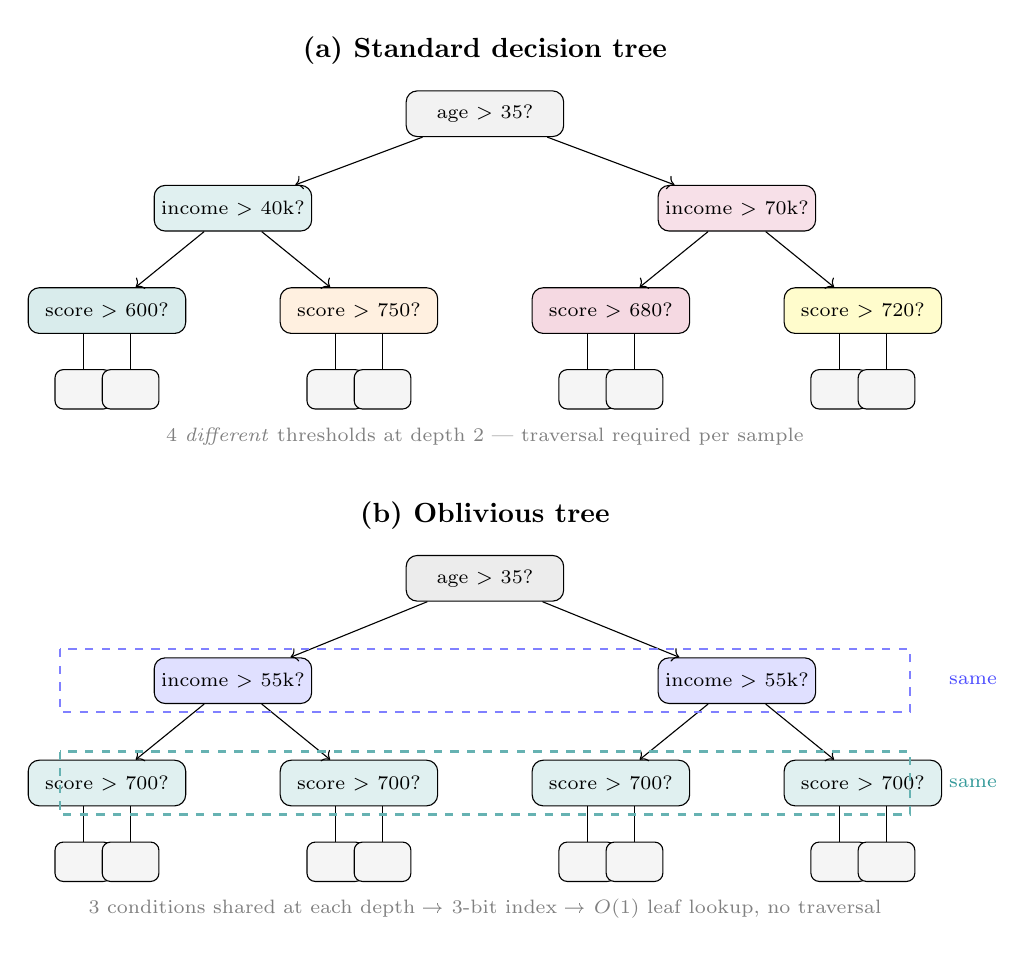
\begin{tikzpicture}[
  every node/.style={font=\small},
  std/.style={draw, rounded corners=4pt, fill=gray!10, minimum width=2.0cm, minimum height=0.58cm, inner sep=2pt, font=\scriptsize},
  obl0/.style={draw, rounded corners=4pt, fill=gray!15, minimum width=2.0cm, minimum height=0.58cm, inner sep=2pt, font=\scriptsize},
  obl1/.style={draw, rounded corners=4pt, fill=blue!12, minimum width=2.0cm, minimum height=0.58cm, inner sep=2pt, font=\scriptsize},
  obl2/.style={draw, rounded corners=4pt, fill=teal!12, minimum width=2.0cm, minimum height=0.58cm, inner sep=2pt, font=\scriptsize},
  leaf/.style={draw, rounded corners=3pt, fill=gray!8, minimum width=0.72cm, minimum height=0.5cm, inner sep=1pt, font=\scriptsize},
]

% ── (a) Standard tree ──
\node[font=\normalsize\bfseries] at (0, 0.5) {(a) Standard decision tree};

\node[std] (r) at (0,-0.3) {age $>$ 35?};

\node[std, fill=teal!12]   (l1) at (-3.2,-1.5) {income $>$ 40k?};
\node[std, fill=purple!12] (l2) at ( 3.2,-1.5) {income $>$ 70k?};

\node[std, fill=teal!15]   (l3) at (-4.8,-2.8) {score $>$ 600?};
\node[std, fill=orange!12] (l4) at (-1.6,-2.8) {score $>$ 750?};
\node[std, fill=purple!15] (l5) at ( 1.6,-2.8) {score $>$ 680?};
\node[std, fill=yellow!20] (l6) at ( 4.8,-2.8) {score $>$ 720?};

\draw[thin,->] (r)  -- (l1); \draw[thin,->] (r)  -- (l2);
\draw[thin,->] (l1) -- (l3); \draw[thin,->] (l1) -- (l4);
\draw[thin,->] (l2) -- (l5); \draw[thin,->] (l2) -- (l6);

\foreach \x in {-5.1,-4.5,-1.9,-1.3, 1.3,1.9, 4.5,5.1}{
  \draw[thin] (\x,-3.09) -- (\x,-3.6);
  \node[leaf] at (\x,-3.8) {};
}

\node[font=\scriptsize, text=gray, align=center] at (0,-4.4)
  {4 \emph{different} thresholds at depth 2 --- traversal required per sample};

% ── (b) Oblivious tree ──
\node[font=\normalsize\bfseries] at (0,-5.4) {(b) Oblivious tree};

\node[obl0] (r2) at (0,-6.2) {age $>$ 35?};

\node[obl1] (m1) at (-3.2,-7.5) {income $>$ 55k?};
\node[obl1] (m2) at ( 3.2,-7.5) {income $>$ 55k?};

\node[obl2] (n1) at (-4.8,-8.8) {score $>$ 700?};
\node[obl2] (n2) at (-1.6,-8.8) {score $>$ 700?};
\node[obl2] (n3) at ( 1.6,-8.8) {score $>$ 700?};
\node[obl2] (n4) at ( 4.8,-8.8) {score $>$ 700?};

\draw[thin,->] (r2) -- (m1); \draw[thin,->] (r2) -- (m2);
\draw[thin,->] (m1) -- (n1); \draw[thin,->] (m1) -- (n2);
\draw[thin,->] (m2) -- (n3); \draw[thin,->] (m2) -- (n4);

\foreach \x in {-5.1,-4.5,-1.9,-1.3, 1.3,1.9, 4.5,5.1}{
  \draw[thin] (\x,-9.09) -- (\x,-9.6);
  \node[leaf] at (\x,-9.8) {};
}

\draw[blue!50, thick, dashed] (-5.4,-7.1) rectangle (5.4,-7.9);
\draw[teal!60, thick, dashed] (-5.4,-8.4) rectangle (5.4,-9.2);
\node[font=\scriptsize, text=blue!70]  at (6.2,-7.5) {same};
\node[font=\scriptsize, text=teal!80]  at (6.2,-8.8) {same};

\node[font=\scriptsize, text=gray, align=center] at (0,-10.4)
  {3 conditions shared at each depth → 3-bit index → $O(1)$ leaf lookup, no traversal};

\end{tikzpicture}
\caption{Standard vs Oblivious tree (depth 3, 8 leaves each).
(a) Standard tree: the same feature \texttt{score} appears at depth 2, but each node uses a \emph{different} threshold (600, 750, 680, 720).
(b) Oblivious tree: every node at the same depth shares an \emph{identical} condition (boxed).
Three shared conditions yield a 3-bit index that directly selects one of $2^3=8$ leaves --- no path traversal needed.}
\label{fig:trees}
\end{figure}

Both trees in Figure~\ref{fig:trees} have the same depth and the same number of leaves.
The visual difference reflects a genuine difference in \textbf{expressiveness}: a standard
tree of depth 3 can use up to $2^3 - 1 = 7$ independent split conditions, while an
Oblivious Tree uses only 3 (one per depth level). This lower flexibility is a deliberate
tradeoff --- it acts as structural regularization, making each tree less prone to
memorising noise. CatBoost compensates by building more trees in the ensemble rather
than making each tree more complex.

\subsection{Structure}

An Oblivious Tree of depth $D$ is defined by $D$ pairs:
\[
\mathrm{splits} = \bigl[(f_0,\,\tau_0),\;(f_1,\,\tau_1),\;\ldots,\;(f_{D-1},\,\tau_{D-1})\bigr]
\]
and $2^D$ leaf values $\{\gamma_j\}_{j=0}^{2^D-1}$.

\subsection{Split Search}

At depth $d$, all $2^d$ existing nodes share the same $(f_d, \tau_d)$.
This shared constraint changes how we search for the best split.

In a standard tree, we find the best split \emph{independently} for each node:
each node looks only at its own samples and picks whatever $(f, \tau)$ maximizes
its local gain. Two sibling nodes can therefore choose completely different
features and thresholds.

In an Oblivious Tree, one $(f, \tau)$ must serve \emph{all} $2^d$ nodes simultaneously.
The natural criterion is to pick the $(f, \tau)$ that maximizes the \emph{total}
gain summed across every node at this depth:

\[
\mathrm{Gain}(f, \tau) = \sum_{n=1}^{2^d}
\left[
  \frac{\Bigl(\sum_{i\in L_n}g_i\Bigr)^2}{\sum_{i\in L_n}h_i}
+ \frac{\Bigl(\sum_{i\in R_n}g_i\Bigr)^2}{\sum_{i\in R_n}h_i}
- \frac{\Bigl(\sum_{i\in n}g_i\Bigr)^2}{\sum_{i\in n}h_i}
\right]
\]

Each bracketed term is the gain from applying $(f, \tau)$ to one node $n$
--- identical in form to the Vanilla GBM gain.
The $\sum_{n=1}^{2^d}$ simply adds these up across all $2^d$ nodes.
A split that helps many nodes a little beats one that helps one node a lot
but hurts the others.

Here $h_i$ is the Hessian (second derivative of loss) --- we will
derive this in Section~\ref{sec:newton}.
For MSE, $h_i = 1$ and each bracketed term reduces exactly to the Vanilla GBM gain.

\begin{listing}[H]
\caption{Oblivious split search (\texttt{tree.py})}
\begin{minted}[linenos, bgcolor=gray!6, fontsize=\small, breaklines]{python}
def _find_split(self, X, g, h, node_indices):
    # node_indices: list of arrays, one per current node,
    #               each containing the sample indices in that node.
    _, F = X.shape
    best_gain, best_f, best_t = 0.0, 0, 0.0

    for j in range(F):                      # try every feature
        # Collect all x-values across all nodes to find thresholds
        all_x     = np.concatenate([X[idx, j] for idx in node_indices])
        unique_x  = np.unique(all_x)
        if len(unique_x) < 2:
            continue
        thresholds = (unique_x[:-1] + unique_x[1:]) / 2.0

        for thresh in thresholds:
            gain_total = 0.0
            valid      = True

            for idx in node_indices:        # SUM over all nodes at this depth
                mask = X[idx, j] <= thresh
                n_L, n_R = mask.sum(), (~mask).sum()
                if n_L < self.min_samples_leaf or n_R < self.min_samples_leaf:
                    valid = False; break

                gL = g[idx][mask].sum();  gR = g[idx][~mask].sum()
                hL = h[idx][mask].sum();  hR = h[idx][~mask].sum()
                gt = g[idx].sum();        ht = h[idx].sum()

                # Newton gain: (sum_g)^2 / sum_h for each side
                gain_total += (gL**2/(hL+1e-9) + gR**2/(hR+1e-9)
                               - gt**2/(ht+1e-9))

            if valid and gain_total > best_gain:
                best_gain, best_f, best_t = gain_total, j, thresh

    return best_f, best_t
\end{minted}
\end{listing}

\subsection{Leaf Value}

After finding all $D$ splits, samples are assigned to $2^D$ leaves.
The leaf value uses the Newton step (Section~\ref{sec:newton}):

\[
\gamma_j = -\frac{\sum_{i \in R_j} g_i}{\sum_{i \in R_j} h_i}
\]

For MSE ($h_i = 1$): $\gamma_j = -\frac{\sum g_i}{|R_j|} = \bar{g}_{R_j}$,
identical to Vanilla GBM.

\begin{listing}[H]
\caption{Leaf value assignment (\texttt{tree.py})}
\begin{minted}[linenos, bgcolor=gray!6, fontsize=\small, breaklines]{python}
n_leaves         = 2 ** self.max_depth
self.leaf_values = np.zeros(n_leaves)
for k, idx in enumerate(node_indices):
    if len(idx) > 0:
        # Newton step: gamma_j = -sum(g) / sum(h)
        # For MSE h=1, this equals mean(y - F) = r-bar (mean pseudo-residual)
        self.leaf_values[k] = -g[idx].sum() / (h[idx].sum() + 1e-9)
\end{minted}
\end{listing}

\subsection{Bit-Index Prediction}

After training, the tree is fully described by two things:
$D$ split conditions $(f_0, \tau_0), \ldots, (f_{D-1}, \tau_{D-1})$,
and an array of $2^D$ leaf values $\gamma_0, \ldots, \gamma_{2^D - 1}$.

To \textbf{predict} for a new sample $x$, we need to find which leaf it
belongs to, then return that leaf's value $\gamma_j$.
In a standard tree, this means traversing the tree from the root:
at each node, check that node's condition and go left or right,
then repeat at the child node, until we reach a leaf.
This takes $O(D)$ steps, and each step depends on the previous one
--- the path is different for every sample.

In an Oblivious Tree, the symmetric structure enables a shortcut.
Because every node at depth $d$ tests the \emph{same} condition $(f_d, \tau_d)$,
we can evaluate all $D$ conditions \emph{independently} and simultaneously.
Each condition produces a single bit $b_d \in \{0, 1\}$:

\[
b_d = \mathbf{1}\!\left[x_{f_d} > \tau_d\right]
\]

The $D$ bits together uniquely identify the leaf --- they are exactly
the sequence of left/right decisions the sample would make at each depth.
Concatenating them as a binary number gives the leaf index directly:

\[
\mathrm{index}(x) = \sum_{d=0}^{D-1} b_d \cdot 2^{D-1-d}
\]

The prediction is then a single array lookup: $h_t(x) = \gamma_{\,\mathrm{index}(x)}$.
No traversal, no branching --- just $D$ comparisons and one table lookup.

This is computed incrementally using left-shift accumulation
(\texttt{index = index * 2 + bit}), which builds the binary integer
one bit at a time from most significant to least significant.

\textbf{Example.} $D=3$, splits evaluate to $(b_0, b_1, b_2) = (1, 0, 1)$:
\[
\mathrm{index} = 0
\xrightarrow{b_0=1} 0\cdot 2 + 1 = 1
\xrightarrow{b_1=0} 1\cdot 2 + 0 = 2
\xrightarrow{b_2=1} 2\cdot 2 + 1 = 5
\]
This sample lands in leaf 5 (out of $2^3 = 8$ leaves),
and its prediction is $\gamma_5$.

The same bit-index calculation appears in two places in the code.
\texttt{predict()} uses it to return leaf values at inference time.
\texttt{get\_leaf\_indices()} uses it during training to tell Ordered Boosting
which leaf each sample falls into (needed for the per-leaf cumulative statistics
in Section~\ref{sec:ordered_boosting}).

\begin{listing}[H]
\caption{Prediction via bit-index (\texttt{tree.py})}
\begin{minted}[linenos, bgcolor=gray!6, fontsize=\small, breaklines]{python}
def predict(self, X):
    indices = np.zeros(len(X), dtype=int)  # start: index = 0 for all samples

    for feature, threshold in self.splits:
        # bit_d = 1 if x[feature] > threshold, else 0
        bit     = (X[:, feature] > threshold).astype(int)
        # Left-shift and append bit: index = index * 2 + bit
        # This builds the binary number d bit at a time.
        indices = indices * 2 + bit

    return self.leaf_values[indices]   # O(1) lookup: no traversal

def get_leaf_indices(self, X):
    # Same logic, but return the integer index instead of the leaf value.
    # Used by Ordered Boosting to track which leaf each sample falls into.
    indices = np.zeros(len(X), dtype=int)
    for feature, threshold in self.splits:
        indices = indices * 2 + (X[:, feature] > threshold).astype(int)
    return indices
\end{minted}
\end{listing}

A standard decision tree traverses a path from root to leaf:
$O(\text{depth})$ conditional checks, each depending on the previous.
An Oblivious Tree evaluates $D$ independent conditions and combines them
with bit arithmetic --- all $D$ conditions can be evaluated \emph{in parallel}
across all samples, making it highly GPU-friendly.

It may seem counterintuitive that more leaves ($2^D$ vs a shallower standard tree)
leads to \emph{faster} prediction. The key insight is that the speed gain
does not come from having fewer leaves, but from \emph{eliminating tree traversal}.
In a standard tree, each sample follows a different path through the nodes,
requiring sequential conditional branching. In an Oblivious Tree,
every sample evaluates the same $D$ conditions --- so the entire dataset
can be processed with $D$ vectorised comparisons followed by a single
array lookup. The $2^D$ leaf table is precomputed at training time
and accessed in $O(1)$ at prediction time, regardless of $D$.

% ═══════════════════════════════════════════════
\section{Ordered Target Statistics}
% ═══════════════════════════════════════════════

\subsection{The Target Leakage Problem}

Many datasets contain categorical features (city, product type, user segment).
A natural way to encode them is \textbf{target statistics}: replace each
category value with the mean target among samples of that category:

\[
\hat{x}_{k,i} = \frac{\displaystyle\sum_{j=1}^N \mathbf{1}[x_{j,i} = x_{k,i}]\cdot y_j}
                     {\displaystyle\sum_{j=1}^N \mathbf{1}[x_{j,i} = x_{k,i}]}
\]

\textbf{The problem:} when computing $\hat{x}_{k,i}$ for sample $k$,
the sum includes $j = k$, i.e.\ the sample's own target $y_k$ is used
to encode its own feature.

\textbf{Concrete example.}
Suppose category ``City A'' has 3 samples with targets $y = 10, 20, 30$.
The encoding for the first sample ($y_1 = 10$) is:
\[
\hat{x}_{1} = \frac{10 + 20 + 30}{3} = 20
\]
At training time the model sees feature value 20 and target 10 --- the
encoding is contaminated by its own label, making the model overconfident
during training but degrading at test time when the sample is absent from
the denominator.

\subsection{Ordered TS: The Fix}

Draw a random permutation $\sigma$ of $\{1,\ldots,N\}$.
For sample $k$ at position $r = \sigma^{-1}(k)$ in the permutation,
use \emph{only} the $r-1$ samples that come \emph{before} $k$ in $\sigma$:

\[
\hat{x}_{k,i} =
\frac{\displaystyle\sum_{\substack{j\,:\;\sigma^{-1}(j) < r \\ x_{j,i}\,=\,x_{k,i}}} y_j
      \;+\; a\cdot p}
{\displaystyle\sum_{\substack{j\,:\;\sigma^{-1}(j) < r \\ x_{j,i}\,=\,x_{k,i}}} 1
      \;+\; a}
\]

\begin{itemize}
  \item $p = \bar{y}$: the global target mean (\textbf{prior}).
  \item $a > 0$: the \textbf{smoothing strength}. When few prior samples
    share the same category as $k$, the estimate defaults toward the
    global mean, preventing noisy estimates from rare categories.
  \item The strict inequality $\sigma^{-1}(j) < r$ ensures $k$ itself
    is \emph{never} included. Leakage is eliminated by construction.
\end{itemize}

\textbf{Critical implementation detail:} the cumulative accumulators
must be updated \emph{after} computing $\hat{x}_{k,i}$, not before.

\begin{listing}[H]
\caption{Ordered TS transform (\texttt{encoder.py})}
\begin{minted}[linenos, bgcolor=gray!6, fontsize=\small, breaklines]{python}
def transform(self, X, y, sigma):
    N     = len(y)
    X_enc = X.astype(float).copy()
    p, a  = self.prior_, self.prior_weight    # prior = mean(y), smoothing a

    for col in self.cat_features:
        cat_sum = defaultdict(float)    # sum of y_j for each category value
        cat_cnt = defaultdict(int)      # count of preceding samples

        for r in range(N):
            k       = sigma[r]           # process samples in permutation order
            cat_val = int(X[k, col])

            # --- STEP 1: compute encoding using ONLY preceding samples ---
            cnt = cat_cnt[cat_val]       # how many j with sigma^{-1}(j) < r
            s   = cat_sum[cat_val]       # sum of y_j for those j

            # x-hat_{k,col} = (sum_y_j + a*p) / (cnt + a)
            X_enc[k, col] = (s + p * a) / (cnt + a)

            # --- STEP 2: update accumulators AFTER encoding (y_k excluded) ---
            cat_sum[cat_val] += y[k]
            cat_cnt[cat_val] += 1

    return X_enc
\end{minted}
\end{listing}

Think of the permutation as a timeline. Sample $k$ arrives at time $r$.
Its categorical encoding is computed from the history up to time $r-1$.
Its own outcome $y_k$ is unknown at that moment, so it is excluded.
This mirrors the real-world situation: at test time, $y_k$ is unknown.

% ═══════════════════════════════════════════════
\section{Ordered Boosting}
\label{sec:ordered_boosting}
% ═══════════════════════════════════════════════

\begin{quote}\small
\textbf{Note.} This section presents an educational approximation of the
CatBoost-style ordered boosting idea. The implementation uses a
permutation-based prefix to reduce self-influence (prediction shift),
but it is not a complete reproduction of CatBoost's production algorithm,
which uses multiple permutations, separate model sets, and additional
engineering. Treat the results as an illustration, not a benchmark.
\end{quote}

\subsection{Gradient Leakage in Standard GBM}

In Vanilla GBM, the positive gradient of sample $k$ at iteration $t$ is:
\[
g_k^t = F_{t-1}(x_k) - y_k
\]
where $F_{t-1}$ was trained on \emph{all $N$ samples including $k$}.
Equivalently, the pseudo-residual is $r_k^t = y_k - F_{t-1}(x_k)$.

Because $F_{t-1}$ has already fitted sample $k$, it predicts closer
to $y_k$ than it would for an unseen sample. This causes $|g_k^t|$
to be \textbf{underestimated} (i.e.\ the pseudo-residual $r_k^t$ is
closer to zero than it should be).

\textbf{Numerical example.} Suppose $y_k = 1.0$.
\begin{itemize}
  \item $F_{t-1}$ trained \emph{including} $k$:
    $F_{t-1}(x_k) = 0.8 \Rightarrow r_k = 0.2$ \quad (biased small)
  \item $F_{t-1}$ trained \emph{excluding} $k$:
    $F_{t-1}(x_k) = 0.5 \Rightarrow r_k = 0.5$ \quad (less biased)
\end{itemize}
The biased pseudo-residual tells the next tree that sample $k$ only needs
a correction of 0.2, when the true correction needed is closer to 0.5.
The model systematically under-corrects its mistakes on training data,
which is a form of overfitting.

\subsection{Ordered Boosting: The Fix}

Draw a random permutation $\sigma$. For sample $k$ at position $r$
in $\sigma$, compute the positive gradient against a model $M_{r-1}^t$ that
was built using only the $r-1$ samples preceding $k$ in $\sigma$:

\[
g_{\sigma(r)}^t = M_{r-1}^t\!\left(x_{\sigma(r)}\right) - y_{\sigma(r)}
\]

Because $M_{r-1}^t$ has never seen $x_{\sigma(r)}$, the gradient estimate
has reduced self-influence compared to Vanilla GBM.
(This is an approximation; the full CatBoost algorithm uses additional mechanisms
to control this bias.)

\subsection{Two Models: $M_{r-1}^t$ versus $F_{t-1}$}

Before deriving the per-leaf approximation, it is worth clarifying why
we need \emph{two} different models in Ordered Boosting, and what each one does.
This is a common point of confusion.

\begin{center}
\begin{tabular}{lll}
\toprule
\textbf{Symbol} & \textbf{Purpose} & \textbf{Updated} \\
\midrule
$F_{t-1}$ & Final ensemble for prediction & Once per iteration (after tree fit) \\
$M_{r-1}^t$ & Gradient estimation only & Once per sample (within iteration) \\
\bottomrule
\end{tabular}
\end{center}

$F_{t-1}$ is the same model used in Vanilla GBM --- the full ensemble
accumulated over the previous $t-1$ iterations. It is used at the
\emph{end} of iteration $t$ to update the prediction:
$F_t = F_{t-1} + \eta \cdot h_t$.

$M_{r-1}^t$ is an auxiliary model used \emph{within} iteration $t$
to compute prefix-corrected gradients. It is built from samples
$\sigma(1), \ldots, \sigma(r-1)$ --- those that appear before sample $k$
in the current permutation. Because $M_{r-1}^t$ has never seen $x_k$,
using it to estimate $g_k^t$ reduces the self-influence that afflicts
Vanilla GBM.

After all gradients $\{g_k^t\}$ are collected, a new tree $h_t$ is fitted
to them and $F_t$ is updated --- exactly as in Vanilla GBM.
The role of $M_{r-1}^t$ ends there; it is an internal tool for
reduced-bias estimation, not part of the final model.

\subsection{Per-Leaf Cumulative Statistics}

Building a separate model for each sample is intractable ($N$ models
per iteration). We approximate $M_{r-1}^t$ using the \emph{previous
iteration's tree} to assign leaf memberships, then accumulate
residuals within each leaf in $\sigma$-order:

\[
M_{r-1}^t(x_k) \approx F_{t-1}(x_k) +
\frac{\displaystyle\sum_{\substack{s<r \\ x_{\sigma(s)}\in R_j}}
      \bigl(y_{\sigma(s)} - F_{t-1}(x_{\sigma(s)})\bigr)}
     {\displaystyle\left|\{s<r : x_{\sigma(s)}\in R_j\}\right|}
\]

where $R_j$ is the leaf of the previous tree containing $x_k$.

In code, $\mathrm{base}_k = F_{t-1}(x_k) - y_k = g_k^t$ (the vanilla positive gradient),
and \texttt{correction} is the mean base of previous samples in the same leaf.
It is worth verifying that \texttt{g[k] = base[k] - correction} is indeed
approximately equal to $M_{r-1}^t(x_k) - y_k$:

\begin{align*}
g_k^{\text{ordered}} &= \mathrm{base}_k - \mathrm{correction}_k \\
    &= \bigl(F_{t-1}(x_k) - y_k\bigr)
       - \underbrace{\bigl(F_{t-1}(x_k) - M_{r-1}^t(x_k)\bigr)}_{\text{correction}} \\
    &\approx M_{r-1}^t(x_k) - y_k
\end{align*}

The correction term $F_{t-1}(x_k) - M_{r-1}^t(x_k)$ is approximated by the
per-leaf running mean of preceding gradients: it measures how much the leaf-level
gradients of preceding samples shift the model's prediction beyond $F_{t-1}$.

\begin{listing}[H]
\caption{Ordered gradient computation (\texttt{boosting.py})}
\begin{minted}[linenos, bgcolor=gray!6, fontsize=\small, breaklines]{python}
class OrderedBoosting:
    def compute_gradients(self, y, F_pred, loss, lr,
                          prev_tree=None, sigma=None, X_enc=None):
        N    = len(y)
        base = loss.gradient(y, F_pred)     # base_k = g_k = F_{t-1}(x_k) - y_k  (positive gradient)

        if prev_tree is not None and X_enc is not None:
            leaf_ids = prev_tree.get_leaf_indices(X_enc)
            n_leaves = prev_tree.n_leaves
        else:
            leaf_ids = np.zeros(N, dtype=int)   # first iteration: all leaf 0
            n_leaves = 1

        leaf_sum = np.zeros(n_leaves)
        leaf_cnt = np.zeros(n_leaves, dtype=int)
        g        = np.empty(N)

        for r in range(N):
            k    = sigma[r]
            li   = leaf_ids[k]
            corr = leaf_sum[li] / leaf_cnt[li] if leaf_cnt[li] > 0 else 0.0
            g[k] = base[k] - corr           # g_k = base_k - correction

            # Update AFTER computing g[k] (k excluded from own correction)
            leaf_sum[li] += base[k]
            leaf_cnt[li] += 1

        h = loss.hessian(y, F_pred)
        return g, h
\end{minted}
\end{listing}

This is the same idea as Ordered TS, applied to gradient estimation.
In Ordered TS, sample $k$'s feature encoding excludes its own $y_k$.
In Ordered Boosting, sample $k$'s gradient excludes its own contribution
to the model. Both prevent a sample from ``seeing'' its own label.

\begin{algorithm}[t]
\caption{CatBoost-style ordered boosting with Oblivious Trees (educational approximation)}
{\small
\begin{algorithmic}[1]
\Require $\{(x_i, y_i)\}_{i=1}^N$,\; $\eta$,\; $T$,\; depth $D$,\; smoothing $a$
\State $F_0(x) \leftarrow \bar{y}$;\enspace $h_0 \leftarrow \mathrm{None}$
\For{$t = 1, 2, \ldots, T$}
  \State \textbf{// Step 1: fresh permutation}
  \State $\sigma \leftarrow \mathrm{RandomPermutation}(N)$
  \State \textbf{// Step 2: Ordered TS --- encode categorical features}
  \State $S_c \leftarrow 0,\; C_c \leftarrow 0$ for every category $c$
  \For{$r = 1, \ldots, N$}
    \State $k \leftarrow \sigma(r)$
    \For{each categorical feature $i$}
      \State $c \leftarrow x_{k,i}$;\enspace
        $\hat{x}_{k,i} \leftarrow (S_c + a\bar{y})\,/\,(C_c + a)$
        \hfill\Comment{only preceding samples; $k$ excluded}
      \State $S_c \mathrel{+}= y_k$;\enspace $C_c \mathrel{+}= 1$
        \hfill\Comment{update AFTER encoding}
    \EndFor
  \EndFor
  \State $\tilde{x}_i \leftarrow$ encoded features of sample $i$
  \State \textbf{// Step 3: Ordered Boosting --- prefix-corrected gradients}
  \State $j_i \leftarrow$ leaf of $h_{t-1}$ for $\tilde{x}_i$
    \hfill\Comment{$h_0{=}\mathrm{None}$: all $j_i{\leftarrow}0$}
  \State $A_j \leftarrow 0,\; N_j \leftarrow 0$ for $j = 0,\ldots,2^D-1$
  \For{$r = 1, \ldots, N$}
    \State $k \leftarrow \sigma(r)$;\enspace $j \leftarrow j_k$
    \State $b_k \leftarrow \partial L/\partial F\,(y_k,\,F_{t-1}(\tilde{x}_k))$;\enspace
      $\delta \leftarrow A_j/N_j$ if $N_j{>}0$ else $0$
    \State $g_k^t \leftarrow b_k - \delta$
      \hfill\Comment{prefix-corrected: $\approx\partial L/\partial F\,(y_k,\,M_{r-1}^t(\tilde{x}_k))$}
    \State $A_j \mathrel{+}= b_k$;\enspace $N_j \mathrel{+}= 1$
      \hfill\Comment{update AFTER; $k$ excluded from own correction}
  \EndFor
  \State $h_i^t \leftarrow \partial^2 L/\partial F^2\,(y_i,\,F_{t-1}(\tilde{x}_i))$
    \hfill\Comment{Hessian; $=1$ for MSE}
  \State \textbf{// Step 4: fit one Oblivious Tree}
  \State All $N$ samples in root;\enspace $\mathrm{splits} \leftarrow []$
  \For{$d = 1, \ldots, D$}
    \State $(f^*, \tau^*) \leftarrow \operatorname{arg\,max}_{f,\tau}
      \sum_{n}\!
      \bigl[\tfrac{G_{L_n}^2}{H_{L_n}}+\tfrac{G_{R_n}^2}{H_{R_n}}-\tfrac{G_n^2}{H_n}\bigr]$
      \hfill\Comment{one split shared across ALL $2^{d-1}$ nodes}
    \State $\mathrm{splits}.\mathrm{append}(f^*,\tau^*)$;\enspace
      split every node on $\tilde{x}_{f^*}$ vs $\tau^*$
  \EndFor
  \State $\gamma_j \leftarrow -G_j/H_j$ for each leaf $j$
    \hfill\Comment{$G_j{=}\sum_{i\in j}g_i^t$,\; $H_j{=}\sum_{i\in j}h_i^t$}
  \State $h_t(x) \leftarrow \gamma_{\mathrm{idx}(x)}$,\quad
    $\mathrm{idx}(x)=\sum_{d=0}^{D-1}\mathbf{1}[\tilde{x}_{f_d}{>}\tau_d]\cdot 2^{D-1-d}$
    \hfill\Comment{bit-index}
  \State \textbf{// Step 5: update ensemble}
  \State $F_t(x) \leftarrow F_{t-1}(x)+\eta\cdot h_t(x)$;\enspace
    $h_{t-1} \leftarrow h_t$
\EndFor
\State \Return $F_T$
\end{algorithmic}
}
\end{algorithm}

\textbf{Two nested loops, two different roles.}
It is easy to lose track of what the two $\sigma$-order loops (Steps 2 and 3)
are doing. They share the same permutation $\sigma$ but serve completely
different purposes:

\begin{center}
\begin{tabular}{lll}
\toprule
\textbf{Loop} & \textbf{What it computes} & \textbf{Accumulates} \\
\midrule
Step 2 (Ordered TS) & $\hat{x}_{k,i}$: categorical encoding of features & $S_c, C_c$ per category \\
Step 3 (Ordered Boosting) & $g_k^t$: prefix-corrected gradient & $A_j, N_j$ per leaf \\
\bottomrule
\end{tabular}
\end{center}

Both loops follow the same invariant: \emph{compute first, update after}.
This single rule is what prevents sample $k$ from appearing in its own
encoding (Step 2) or its own gradient correction (Step 3).

\subsection{When Does Ordered Boosting Actually Help?}
\label{sec:ordered_practical}

Ordered TS and Ordered Boosting solve \emph{different} leakage problems,
and it is important to keep them separate.

\textbf{Ordered TS} is specific to categorical features.
When a category's encoding uses the sample's own $y_k$, the encoded feature
becomes a direct function of the target --- a strong and direct form of leakage.
Without categorical features, Ordered TS is simply not needed.

\textbf{Ordered Boosting} addresses gradient leakage, which exists regardless
of feature type. Even with purely numerical features, $F_{t-1}$ was trained
on all $N$ samples including $k$, so $F_{t-1}(x_k)$ is biased toward $y_k$,
causing $g_k^t$ to be underestimated. This is a real problem.

However, the \emph{magnitude} of the two leakages is very different.
In Ordered TS, sample $k$'s own $y_k$ appears directly in the numerator
of its feature encoding --- a first-order effect.
In Ordered Boosting with numerical features, the bias in $F_{t-1}(x_k)$
is a weaker, indirect effect: the model has seen $x_k$ during training,
but shares it with $N-1$ other samples, so the per-sample influence is
$O(1/N)$.

In practice, this means:

\begin{itemize}
  \item \textbf{Numerical features only, large dataset} ---
    Ordered Boosting provides marginal benefit.
    Plain mode is faster and often equally accurate.

  \item \textbf{Categorical features present} ---
    Ordered TS eliminates a strong leakage source, and Ordered Boosting
    should be used alongside it (the paper requires $\sigma_{\mathrm{cat}} = \sigma_{\mathrm{boost}}$
    to guarantee full leakage removal).

  \item \textbf{Small dataset, numerical only} ---
    Ordered Boosting can still reduce overfitting, since the per-sample
    influence of $O(1/N)$ is larger when $N$ is small.

  \item \textbf{External walk-forward validation already applied} ---
    If the training pipeline already prevents look-ahead bias at the split
    level (e.g.\ time-series walk-forward retraining), Ordered Boosting
    adds little on top.
\end{itemize}

The CatBoost documentation reflects this: Ordered mode is recommended
for small datasets, while Plain mode is the default for large ones.
For datasets with only numerical features and an existing temporal validation
structure, Plain mode with other regularization (e.g.\ posterior sampling,
Section~\ref{sec:sglb}) is often the better choice.

% ═══════════════════════════════════════════════
\section{Posterior Sampling via Stochastic Gradient Langevin Boosting}
\label{sec:sglb}
% ═══════════════════════════════════════════════

\subsection{Motivation: From Point Estimate to Distribution}

Vanilla GBM finds a single model $F^*$ that minimizes the loss:

\[
F^* = \operatorname{arg\,min}_F \sum_{i=1}^N L(y_i, F(x_i))
\]

This is a point estimate. It tells us \emph{what} to predict, but not
\emph{how confident} we should be. Three problems remain unaddressed:

\begin{itemize}
  \item \textbf{Local minima.} When the loss landscape is non-convex,
    $F^*$ may be a local rather than global minimum. Standard GBM has no
    mechanism to escape.
  \item \textbf{Overfitting.} Gradient boosting aggressively fits the
    training data. Without explicit regularization, $F^*$ memorizes noise.
    Previous chapters addressed this structurally (Oblivious Trees,
    Ordered Boosting); SGLB adds a complementary stochastic regularization:
    noise injection prevents the model from converging too precisely to
    any single point, acting similarly to dropout in neural networks.
  \item \textbf{Uncertainty.} For a new sample $x$, how much should we
    trust the prediction $F^*(x)$? A point estimate gives no answer.
\end{itemize}

All three are addressed by replacing the point estimate with a
\textbf{posterior distribution} over functions $p(F|\mathcal{D})$.

\subsection{Langevin Dynamics}

Langevin dynamics adds noise to gradient descent:

\[
\theta_{t+1} = \theta_t - \eta\,\nabla L(\theta_t) + \sqrt{\frac{2\eta}{\beta}}\,\epsilon_t,
\quad \epsilon_t \sim \mathcal{N}(0, I)
\]

The noise term $\sqrt{2\eta/\beta}\,\epsilon_t$ allows the algorithm to
escape local minima --- it performs a gradient-biased random walk rather
than pure gradient descent.

The key theoretical result (via the Fokker-Planck equation) is that
this Markov chain converges in distribution to:

\[
p(\theta) \propto \exp(-\beta\,L(\theta))
\]

This is a \textbf{Boltzmann distribution}: states with low loss have
high probability, states with high loss have low probability.
$\beta$ is the \emph{inverse temperature} --- large $\beta$ concentrates
the distribution near the minimum (approaching MAP), small $\beta$ spreads
it broadly.

\subsection{Connection to the Posterior}

If we define loss as negative log-likelihood,
$L(F) = -\log p(\mathcal{D}|F)$, and assume a uniform prior, then:

\[
p(F|\mathcal{D}) \propto p(\mathcal{D}|F) \cdot p(F) = \exp(-L(F))
\]

The stationary distribution of Langevin dynamics is exactly the
\textbf{Bayesian posterior} over $F$.
Gradient descent finds the posterior mode (MAP);
Langevin dynamics \emph{samples} from the full posterior.

\subsection{SGLB: Applying Langevin Dynamics to Boosting}

Applying Langevin dynamics to function space gives
\textbf{Stochastic Gradient Langevin Boosting} (SGLB,
Ustimenko \& Prokhorenkova, 2021).
Three changes from Vanilla GBM:

\begin{enumerate}
  \item \textbf{Noise injection.} Add Langevin noise to positive gradients:
    \[
      \tilde{g}_k^t = g_k^t + \epsilon_k, \quad
      \epsilon_k \sim \mathcal{N}\!\left(0,\;\frac{2\eta}{\beta}\right)
    \]

  \item \textbf{Noisy tree fit.} Fit the tree to $\tilde{g}^t$ instead of $g^t$:
    \[
      h_t = \operatorname{FitTree}(X,\, \tilde{g}^t)
    \]

  \item \textbf{Shrinkage update.} Apply L2-style weight decay to $F$:
    \[
      F_t = (1 - \alpha\eta)\,F_{t-1} + \eta\cdot h_t(x)
    \]
    The shrinkage term $(1-\alpha\eta)$ ensures the stationary distribution
    is normalizable for any loss function:
    \[
      p(F) \propto \exp\!\left(-\beta\left(L(F) + \frac{\alpha}{2}\|F\|^2\right)\right)
    \]
\end{enumerate}

\textbf{Why shrinkage is necessary.}
Without shrinkage, the stationary distribution $\exp(-\beta L(F))$
may not be normalizable --- for example, if $L(F) \to 0$ as
$F \to -\infty$ (as with exponential-family losses), the integral
$\int \exp(-\beta L(F))\,dF$ diverges.
The $\frac{\alpha}{2}\|F\|^2$ term guarantees integrability
regardless of the loss function.

\begin{listing}[H]
\caption{SGLB gradient and update (\texttt{boosting.py})}
\begin{minted}[linenos, bgcolor=gray!6, fontsize=\small, breaklines]{python}
class SGLB:
    def __init__(self, alpha=0.01, beta=100.0, rng=None):
        self.alpha = alpha          # shrinkage strength
        self.beta  = beta           # inverse temperature
        self.rng   = rng or np.random.default_rng()

    def compute_gradients(self, y, F_pred, loss, lr,
                          prev_tree=None, sigma=None, X_enc=None):
        g = loss.gradient(y, F_pred)
        h = loss.hessian(y, F_pred)

        # [*1] Langevin noise:  epsilon ~ N(0, sqrt(2*lr/beta))
        sigma_noise = np.sqrt(2.0 * lr / self.beta)
        g = g + self.rng.normal(0.0, sigma_noise, size=g.shape)
        return g, h

    def update(self, F_pred, tree_pred, lr):
        # [*3] shrinkage: F_t = (1 - alpha*lr)*F_{t-1} + lr*h_t
        return (1.0 - self.alpha * lr) * F_pred + lr * tree_pred
\end{minted}
\end{listing}

\subsection{Epistemic Uncertainty via Posterior Sampling}

A single SGLB run can be interpreted as producing an approximate
posterior-like sample.
To estimate \textbf{epistemic uncertainty} (heuristically), run $S$ independent
chains (different random seeds) and compute the variance of predictions:

\[
\hat{\mu}(x) = \frac{1}{S}\sum_{s=1}^S F^{(s)}(x), \qquad
\hat{\sigma}^2(x) = \frac{1}{S}\sum_{s=1}^S \bigl(F^{(s)}(x) - \hat{\mu}(x)\bigr)^2
\]

$\hat{\sigma}^2(x)$ is large when the $S$ models disagree --- indicating
that the data does not strongly constrain the prediction at $x$.
This variance is used as a \textbf{heuristic proxy for epistemic uncertainty}:
the intuition is that it should decrease as more data constrains the model,
unlike aleatoric uncertainty (irreducible data noise), though the connection
to true Bayesian posterior uncertainty is approximate.

\begin{listing}[H]
\caption{Epistemic uncertainty via ensemble (\texttt{model.py})}
\begin{minted}[linenos, bgcolor=gray!6, fontsize=\small, breaklines]{python}
# SGLBEnsemble acts as a factory only (boosting.py)
class SGLBEnsemble:
    def make_sglb(self, seed) -> SGLB:
        return SGLB(alpha=self.alpha, beta=self.beta,
                    rng=np.random.default_rng(seed))

# GradientBoosting trains S independent models, stores tree_sets (model.py)
# fit():
for seed in self.boosting.seeds:
    sglb  = self.boosting.make_sglb(seed)
    trees = self._fit_single(X, y, sglb, rng=np.random.default_rng(seed))
    self.tree_sets.append(trees)

# predict_uncertainty():
preds = np.stack(
    [self._predict_single(X_enc, trees, self.boosting.make_sglb(s))
     for trees, s in zip(self.tree_sets, self.boosting.seeds)],
    axis=0,
)                           # (S, N)
return preds.var(axis=0)    # epistemic uncertainty
\end{minted}
\end{listing}

\subsection{Practical Considerations}

\textbf{Comparison with Random Forest variance.}
RF uncertainty is also estimated via ensemble variance, but the source
of diversity is bootstrap sampling and feature subsampling.
SGLB diversity comes from Langevin noise in gradient space.
Both share the same structural limitation for tree-based models:
extrapolation regions (out-of-distribution $x$) collapse to the nearest
leaf, so all models agree and variance drops to zero.
Within the training distribution, SGLB variance and RF variance capture
similar epistemic uncertainty and tend to be highly correlated.

\textbf{Comparison with aleatoric uncertainty (RMSEWithUncertainty).}
RMSEWithUncertainty trains a single model to jointly predict $\mu(x)$
and $\sigma^2(x)$ by minimizing the Gaussian negative log-likelihood:
$L = \frac{(y-\mu)^2}{2\sigma^2} + \frac{1}{2}\log\sigma^2$.
This $\sigma^2(x)$ measures \emph{data noise} --- it does not decrease
with more data. SGLB $\hat{\sigma}^2(x)$ measures \emph{model uncertainty}
and does decrease with more data.

\textbf{Cost.} $S$ independent SGLB runs multiply training time by $S$.
For monthly retraining with moderate $N$, $S = 10$--$20$ is practical.

\textbf{When to use SGLB instead of Ordered Boosting.}
For datasets with only numerical features and an existing walk-forward
validation structure, Plain mode + SGLB provides regularization
(via shrinkage and noise) and uncertainty estimation without the
computational overhead of Ordered Boosting.

% ═══════════════════════════════════════════════
\section{Module Architecture}
% ═══════════════════════════════════════════════

The implementation is split into five modules, each with a single responsibility:

\begin{center}
\begin{tabular}{lll}
\toprule
\textbf{Module} & \textbf{Class / Function} & \textbf{Responsibility} \\
\midrule
\texttt{tree.py} & \texttt{ObliviousTree} & Split search, bit-index prediction \\
\texttt{loss.py} & \texttt{MSE}, \texttt{LogLoss} & Gradient, Hessian, leaf value \\
\texttt{ordered\_ts.py} & \texttt{OrderedTS} & Categorical feature encoding \\
\texttt{ordered\_boost.py} & \texttt{ordered\_gradients\_from\_leaf\_ids} & Per-leaf gradient estimation \\
\texttt{model.py} & \texttt{CatBoostScratch} & Assembly only --- no logic \\
\bottomrule
\end{tabular}
\end{center}

\texttt{model.py} sequences the modules in the correct order and holds
no algorithmic logic of its own. Each module is independently testable.

\begin{listing}[H]
\caption{Training loop in \texttt{model.py} (\texttt{\_fit\_single}, simplified)}
\begin{minted}[linenos, bgcolor=gray!6, fontsize=\small, breaklines]{python}
def _fit_single(self, X, y, boosting_strategy, rng):
    N, F_pred = len(y), np.full(len(y), self.F0)
    trees, prev_tree = [], None

    for _ in range(self.n_estimators):
        sigma = rng.permutation(N)

        # (a) Ordered TS: encode categorical features using permutation sigma
        X_enc = self._ts_enc.transform(X, y, sigma) if self.cat_features else X

        # (b) gradient + hessian via boosting strategy
        g, h = boosting_strategy.compute_gradients(
            y, F_pred, self.loss, self.learning_rate,
            prev_tree=prev_tree, sigma=sigma, X_enc=X_enc,
        )

        # (c) fit tree on permuted samples
        tree = self.tree_cls(max_depth=self.max_depth,
                             min_samples_leaf=self.min_samples_leaf,
                             ).fit(X_enc[sigma], g[sigma], h[sigma])

        # (d) update ensemble
        F_pred    = boosting_strategy.update(F_pred, tree.predict(X_enc),
                                             self.learning_rate)
        prev_tree = tree
        trees.append(tree)
    return trees
\end{minted}
\end{listing}

% ═══════════════════════════════════════════════
\section{Experiments}
% ═══════════════════════════════════════════════

\subsection{Setup}

We test on a synthetic regression problem:
\[
y = x_0^2 + 0.5\,x_1 + \varepsilon,\quad
x \sim \mathrm{Uniform}(-3, 3)^2,\quad
\varepsilon \sim \mathcal{N}(0,\, 0.09)
\]
with $N = 400$ samples (train 300, test 100), 100 estimators, $\eta = 0.1$,
depth $= 4$. The noise variance $\sigma^2 = 0.09$ is the irreducible
error floor --- no model can achieve lower test MSE in expectation.
A baseline that predicts the training mean achieves MSE $\approx 7.7$.

All six combinations share the same modular \texttt{GradientBoosting}
interface:
\begin{minted}[linenos, bgcolor=gray!6, fontsize=\small, breaklines]{python}
model = GradientBoosting(
    tree=ObliviousTree, loss=MSE(), boosting=OrderedBoosting(), ...
)
\end{minted}

\subsection{Results}

\begin{center}
\begin{tabular}{llcc}
\toprule
\textbf{\#} & \textbf{Configuration} & \textbf{Train MSE} & \textbf{Test MSE} \\
\midrule
1 & DecisionTree + MSE + Vanilla        & 0.0186 & 0.1798 \\
2 & ObliviousTree + MSE + Vanilla       & 0.0878 & 0.2294 \\
3 & ObliviousTree + MSE + Ordered       & 0.0786 & 0.1718 \\
4 & ObliviousTree + LogLoss + Ordered   & 0.0110 & 0.0694 \\
5 & ObliviousTree + MSE + SGLB          & 0.1089 & 0.2540 \\
6 & ObliviousTree + MSE + SGLBEnsemble  & 0.1038 & 0.2562 \\
\bottomrule
\end{tabular}
\end{center}

Configuration 6 additionally reports epistemic uncertainty:
train $= 0.00258$, test $= 0.00371$ (test 44\% higher).

\subsection{Analysis}

\textbf{\#1 (DecisionTree + Vanilla): severe overfitting.}
Train MSE $0.0186 \ll 0.09$ (noise floor) --- the asymmetric tree
memorizes the training data almost perfectly.
Test MSE $0.1798$ is twice the noise floor, suggesting that the
flexibility that enables tight training fit hurts generalization.

\textbf{\#2 vs \#1 (ObliviousTree): lower expressiveness, not always better.}
Symmetric splits constrain each depth level to a single condition,
raising train MSE to $0.0878$ (closer to the noise floor).
However, test MSE $0.2294$ is \emph{worse} than \#1.
With only 100 estimators, the Oblivious Tree has not converged ---
its expressiveness limit acts more like underfitting than regularization.
With more iterations this ordering may change, but should be tested.

\textbf{\#2 $\to$ \#3 (Ordered Boosting): 25\% test MSE reduction.}
Train MSE changes slightly ($0.0878 \to 0.0786$), while test MSE
drops from $0.2294$ to $0.1718$ --- a 25\% improvement.
This is the core effect of Ordered Boosting: the per-leaf cumulative
correction removes the portion of each gradient already ``explained''
by preceding samples, using prefix-corrected gradient estimates that
reduce self-influence and may generalize better.

\textbf{\#4 (LogLoss + Ordered): classification baseline.}
The target is binarized at the median, giving a balanced 50/50 split.
A random classifier achieves MSE $= 0.25$; the model achieves
$0.0694$ on the test set, suggesting effective learning.
The train/test ratio ($\approx 6\times$) is larger than in regression,
partly because the 0-1 loss surface is non-convex and the model
fits the training labels tightly.

\textbf{\#5--6 (SGLB): regularization at a cost.}
With $\beta = 10$ ($\sigma_\epsilon = \sqrt{2\eta/\beta} = 0.141$),
SGLB raises train MSE to $0.1089$ --- the noise injection prevents
the model from fitting the training set tightly, as intended.
However, test MSE $0.2540$ remains worse than Ordered Boosting ($0.1718$).

The reason is structural: SGLB's benefit (escaping local minima,
stochastic regularization) requires either a multimodal loss landscape
or large $N$. The synthetic target $y = x_0^2 + 0.5x_1 + \varepsilon$
is nearly convex, so there are no local minima to escape.
Ordered Boosting removes a provable bias; SGLB adds beneficial noise
whose advantage depends on the problem geometry.

SGLBEnsemble (\#6) averages 10 independent chains, marginally
reducing variance without changing the bias, giving results nearly
identical to a single SGLB run (\#5).

\textbf{Epistemic uncertainty (\#6): correct ordering.}
Test uncertainty ($0.00371$) exceeds train uncertainty ($0.00258$)
by 44\%.
Test samples lie further from the training distribution's center,
causing the 10 Langevin chains to land in different leaves more often
--- producing higher inter-model variance.
This is consistent with the ensemble variance serving as a proxy for
\emph{epistemic} uncertainty: regions less covered by training data
yield higher prediction disagreement.

\subsection{Summary}

\begin{center}
\begin{tabular}{lp{9cm}}
\toprule
\textbf{Observation} & \textbf{Implication} \\
\midrule
\#1 overtfits, \#2 underconverges &
  Tree choice interacts with iteration budget; symmetric trees need more estimators. \\
\#2 $\to$ \#3 ($-25\%$ test MSE) &
  Ordered Boosting removes a provable gradient bias; benefit is consistent. \\
\#5--6 worse than \#3 &
  SGLB regularization is problem-geometry dependent; use when $N$ is large
  or loss is non-convex. \\
Uncertainty: test $>$ train &
  SGLBEnsemble variance is consistent with epistemic uncertainty interpretation. \\
\bottomrule
\end{tabular}
\end{center}

% ═══════════════════════════════════════════════
\section{Limitations and What We Left Out}
\label{sec:limitations}
% ═══════════════════════════════════════════════

This implementation covers the core ideas but omits several features
present in production CatBoost:

\begin{itemize}
  \item \textbf{Multi-permutation variance reduction.} The original paper
    uses $s$ independent permutations per iteration and averages the
    resulting gradients. This reduces the variance introduced by the
    single-permutation approximation.
  \item \textbf{GPU-optimized split search.} CatBoost's GPU kernel
    exploits the Oblivious Tree structure for fully parallel split evaluation.
  \item \textbf{Advanced categorical handling.} One-hot encoding for
    low-cardinality features, frequency encoding, and combinations.
  \item \textbf{Early stopping and overfitting detector.}
  \item \textbf{Multiclass and ranking losses.}
  \item \textbf{Stochastic Gradient Langevin Boosting (SGLB) and posterior sampling.}
    The \texttt{posterior\_sampling=True} option in CatBoost activates SGLB
    (Ustimenko \& Prokhorenkova, 2021), which modifies the boosting update as:
    \[
      F_t = (1 - \alpha\eta)\,F_{t-1} + \eta\cdot h_t^{\text{noisy}},
      \quad g_k^t \leftarrow g_k^t + \epsilon_k,\;\epsilon_k \sim \mathcal{N}(0,\sigma^2)
    \]
    The shrinkage term $(1-\alpha\eta)$ regularizes the model; the noise
    $\epsilon_k$ injected into each gradient causes the Markov chain of
    models to converge not to a point estimate but to a distribution
    $p(F) \propto \exp(-L(F)/\eta)$, which approximates the posterior over functions
    under a uniform prior (in the continuous-time, infinite-data limit). Running multiple independent chains and averaging
    their predictions yields an approximate Monte-Carlo estimate of posterior variance
    --- a useful but heuristic uncertainty estimate. This is particularly useful when
    Plain mode (no Ordered Boosting) is used with numerical features and
    an external walk-forward validation structure already handles look-ahead
    bias, as the SGLB noise provides regularization without the computational
    overhead of Ordered Boosting.
\end{itemize}

% ═══════════════════════════════════════════════
\section{Conclusion}
% ═══════════════════════════════════════════════

Starting from undergraduate calculus and the idea of gradient descent,
we derived and implemented five innovations that transform Vanilla GBM
into a modern, principled gradient boosting system:

\begin{enumerate}
  \item \textbf{Newton Step} generalizes the leaf value computation via a
    second-order Taylor approximation, enabling any differentiable loss function
    through a unified gradient/Hessian interface.
  \item \textbf{Oblivious Trees} replace standard decision trees with a
    symmetric structure that enables $O(1)$ bit-index prediction and
    efficient GPU parallelism.
  \item \textbf{Ordered Target Statistics} prevent categorical feature encoding
    from leaking the target by conditioning on strictly preceding samples
    in a random permutation.
  \item \textbf{Ordered Boosting} computes CatBoost-style prefix-corrected gradient estimates
    by computing each sample's residual against a model that has never
    seen that sample, implemented efficiently via per-leaf cumulative statistics.
  \item \textbf{Posterior Sampling (SGLB)} injects Langevin noise into
    gradient estimates and applies shrinkage, transforming the boosting
    Markov chain into an approximate posterior sampler over functions.
    Running $S$ independent chains yields heuristic epistemic uncertainty estimates
    via Monte-Carlo variance.
\end{enumerate}

Each innovation is independently testable and motivated by a concrete
limitation of the previous approach. The experimental results are consistent
with the theoretical predictions: Ordered Boosting reduces test MSE by
reducing gradient self-influence, and SGLB uncertainty estimates
assign higher variance to out-of-distribution regions within the
training support.

\begin{thebibliography}{9}
\bibitem{catboost}
Prokhorenkova, L., Gusev, G., Vorobev, A., Dorogush, A.~V., \& Gulin, A. (2018).
\textit{CatBoost: unbiased boosting with categorical features}.
Advances in Neural Information Processing Systems (NeurIPS), 31.

\bibitem{friedman}
Friedman, J.~H. (2001).
\textit{Greedy function approximation: a gradient boosting machine}.
Annals of Statistics, 29(5), 1189--1232.
\end{thebibliography}

\end{document}
